\documentclass[12pt]{article}
\usepackage{graphicx}
\usepackage{wrapfig}
\usepackage[margin=0.5in]{geometry}
\usepackage[utf8]{inputenc}
\usepackage{amsmath, amsthm, amssymb}
\usepackage{txfonts}
\usepackage{verbatim}
\usepackage{multirow}
\usepackage{booktabs}
\usepackage{float}
\usepackage{indentfirst}
\usepackage{tikz}
\usepackage[font={small,it}]{caption}
\usetikzlibrary{shapes,arrows}
\usepackage{float}
\setcounter{secnumdepth}{5}   
\setcounter{tocdepth}{5}

\usepackage{eso-pic}
\newcommand\BackgroundPic{
\put(0,0){
\parbox[b][\paperheight]{\paperwidth}{%
\centering
\vspace{10 mm}
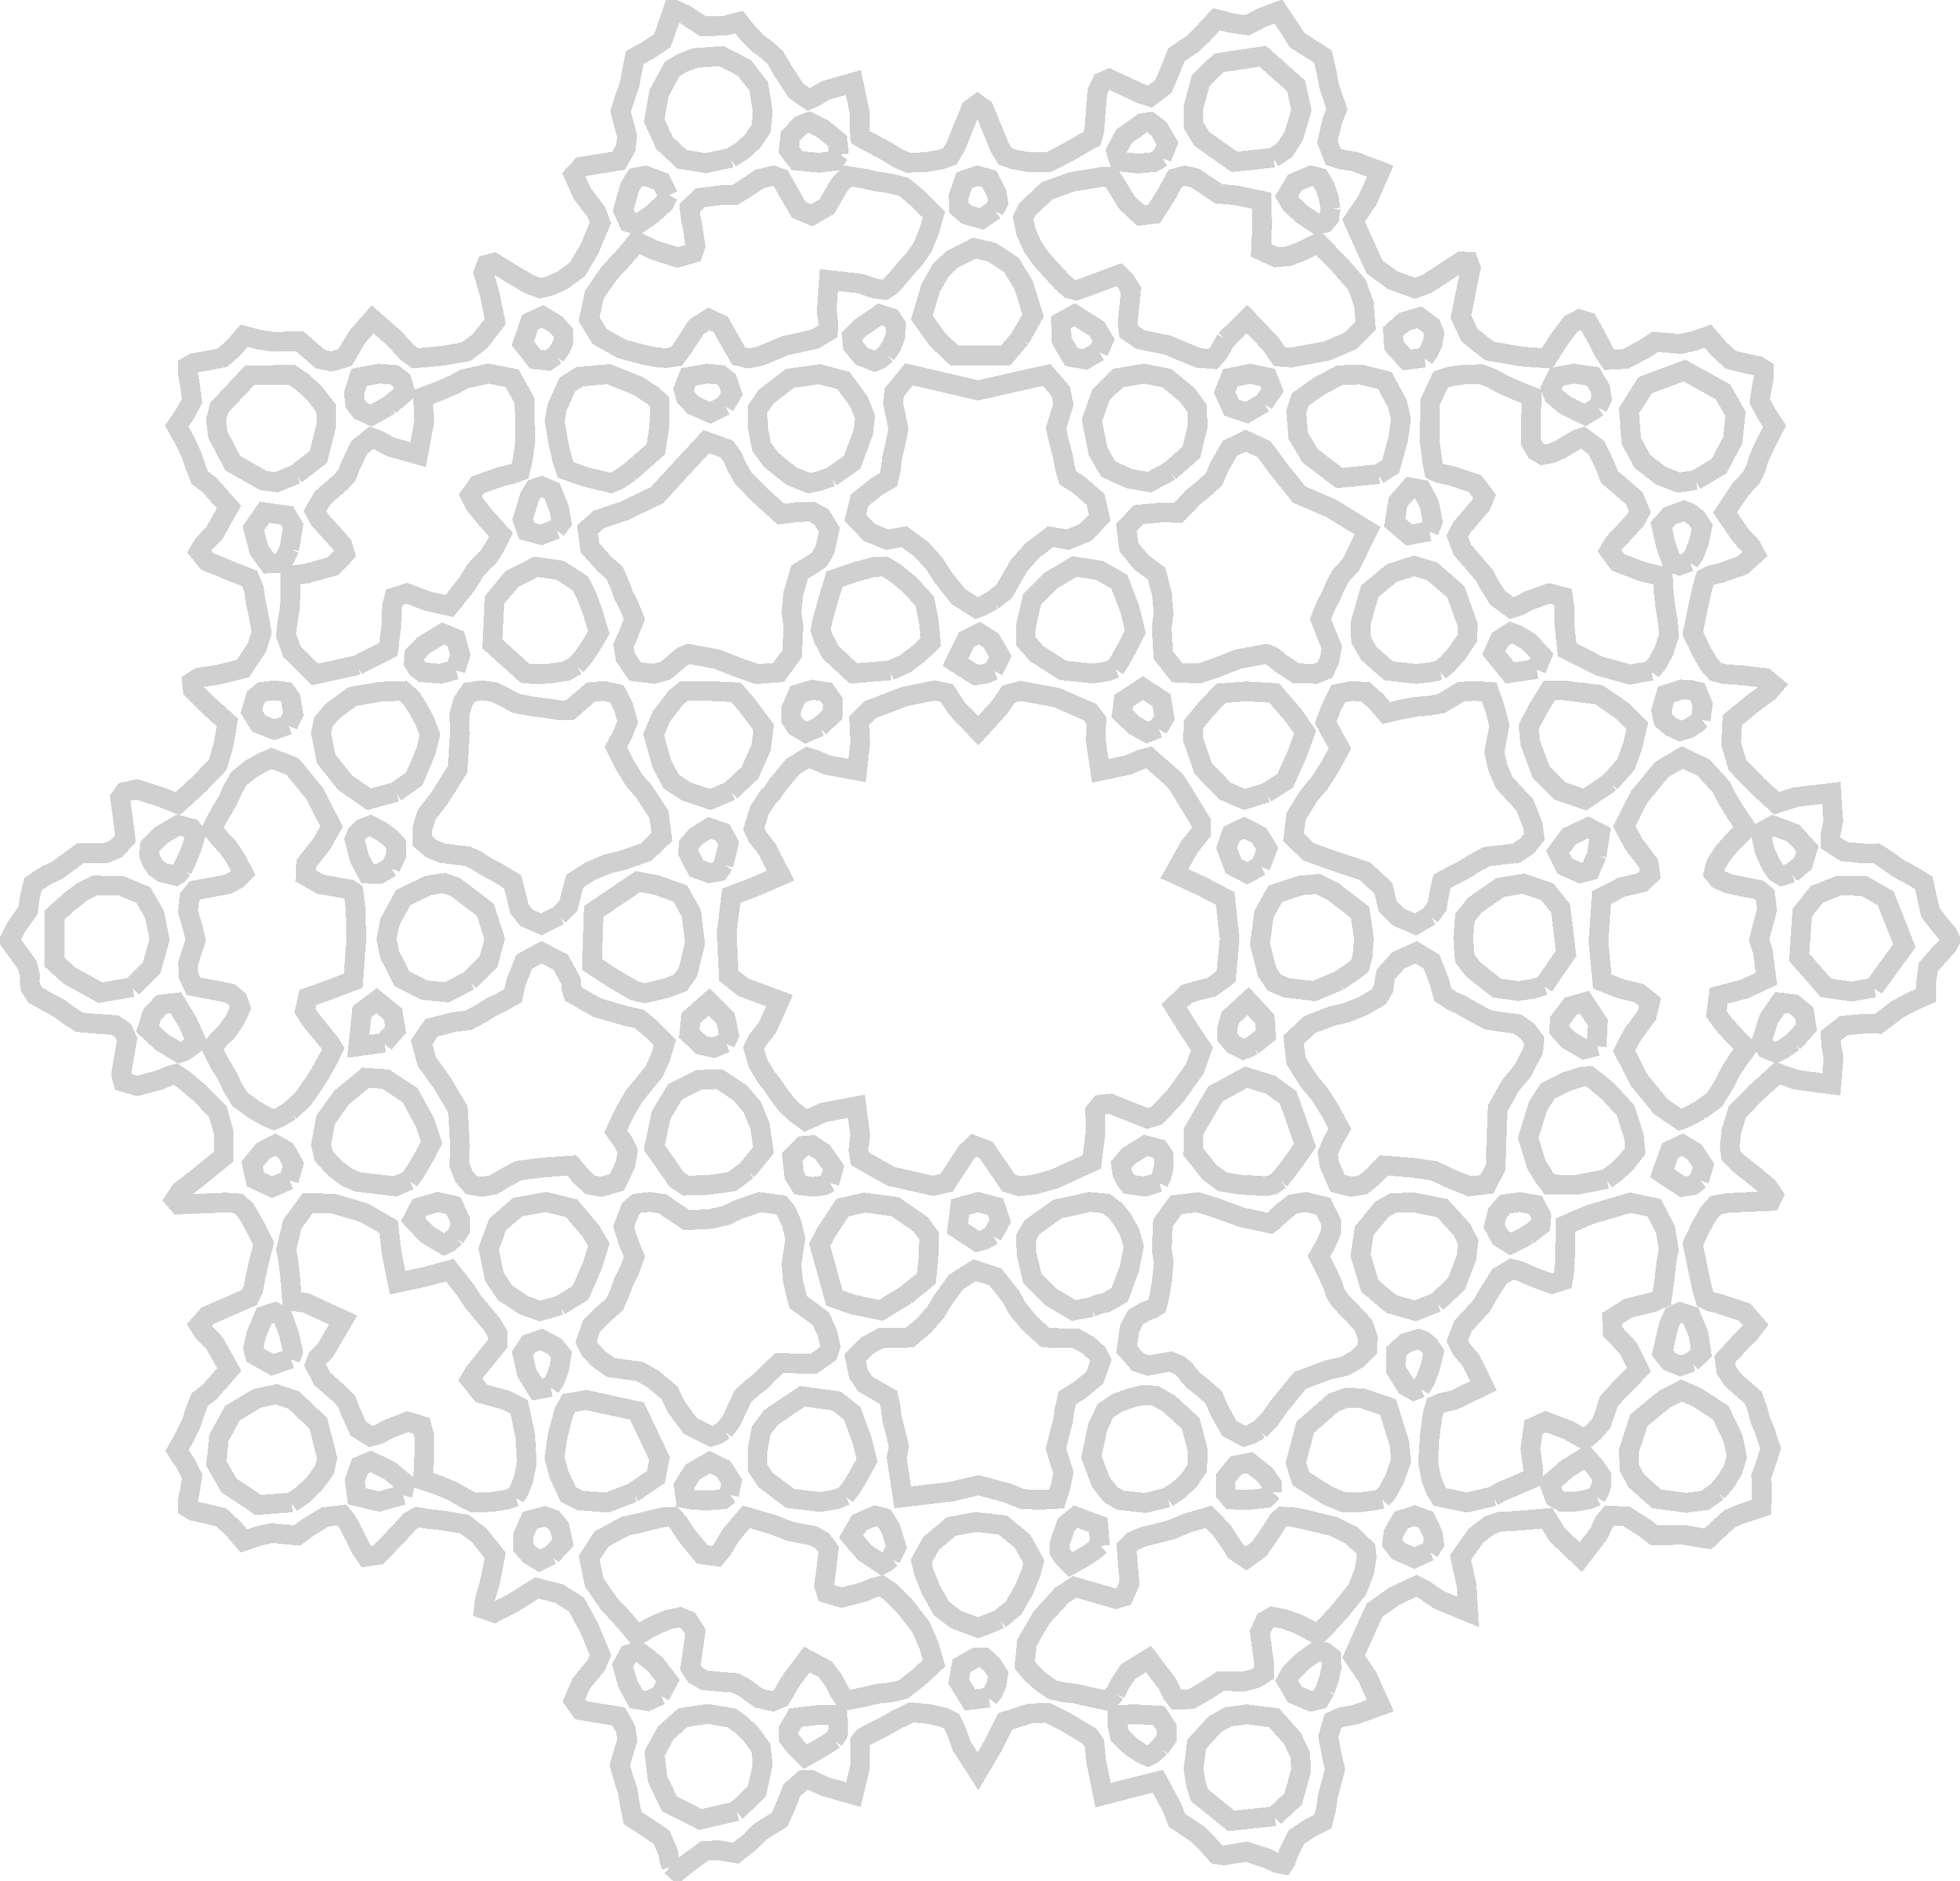
\includegraphics[width=\paperwidth,height=.14\paperheight,
keepaspectratio]{qq552.pdf}%
\vfill
}}}

\newcommand{\HRule}{\rule{\linewidth}{0.5mm}}
\setlength{\parindent}{.0in}
\begin{document}
\thispagestyle{empty}
\thispagestyle{empty}
\begin{minipage}{0.12\textwidth}
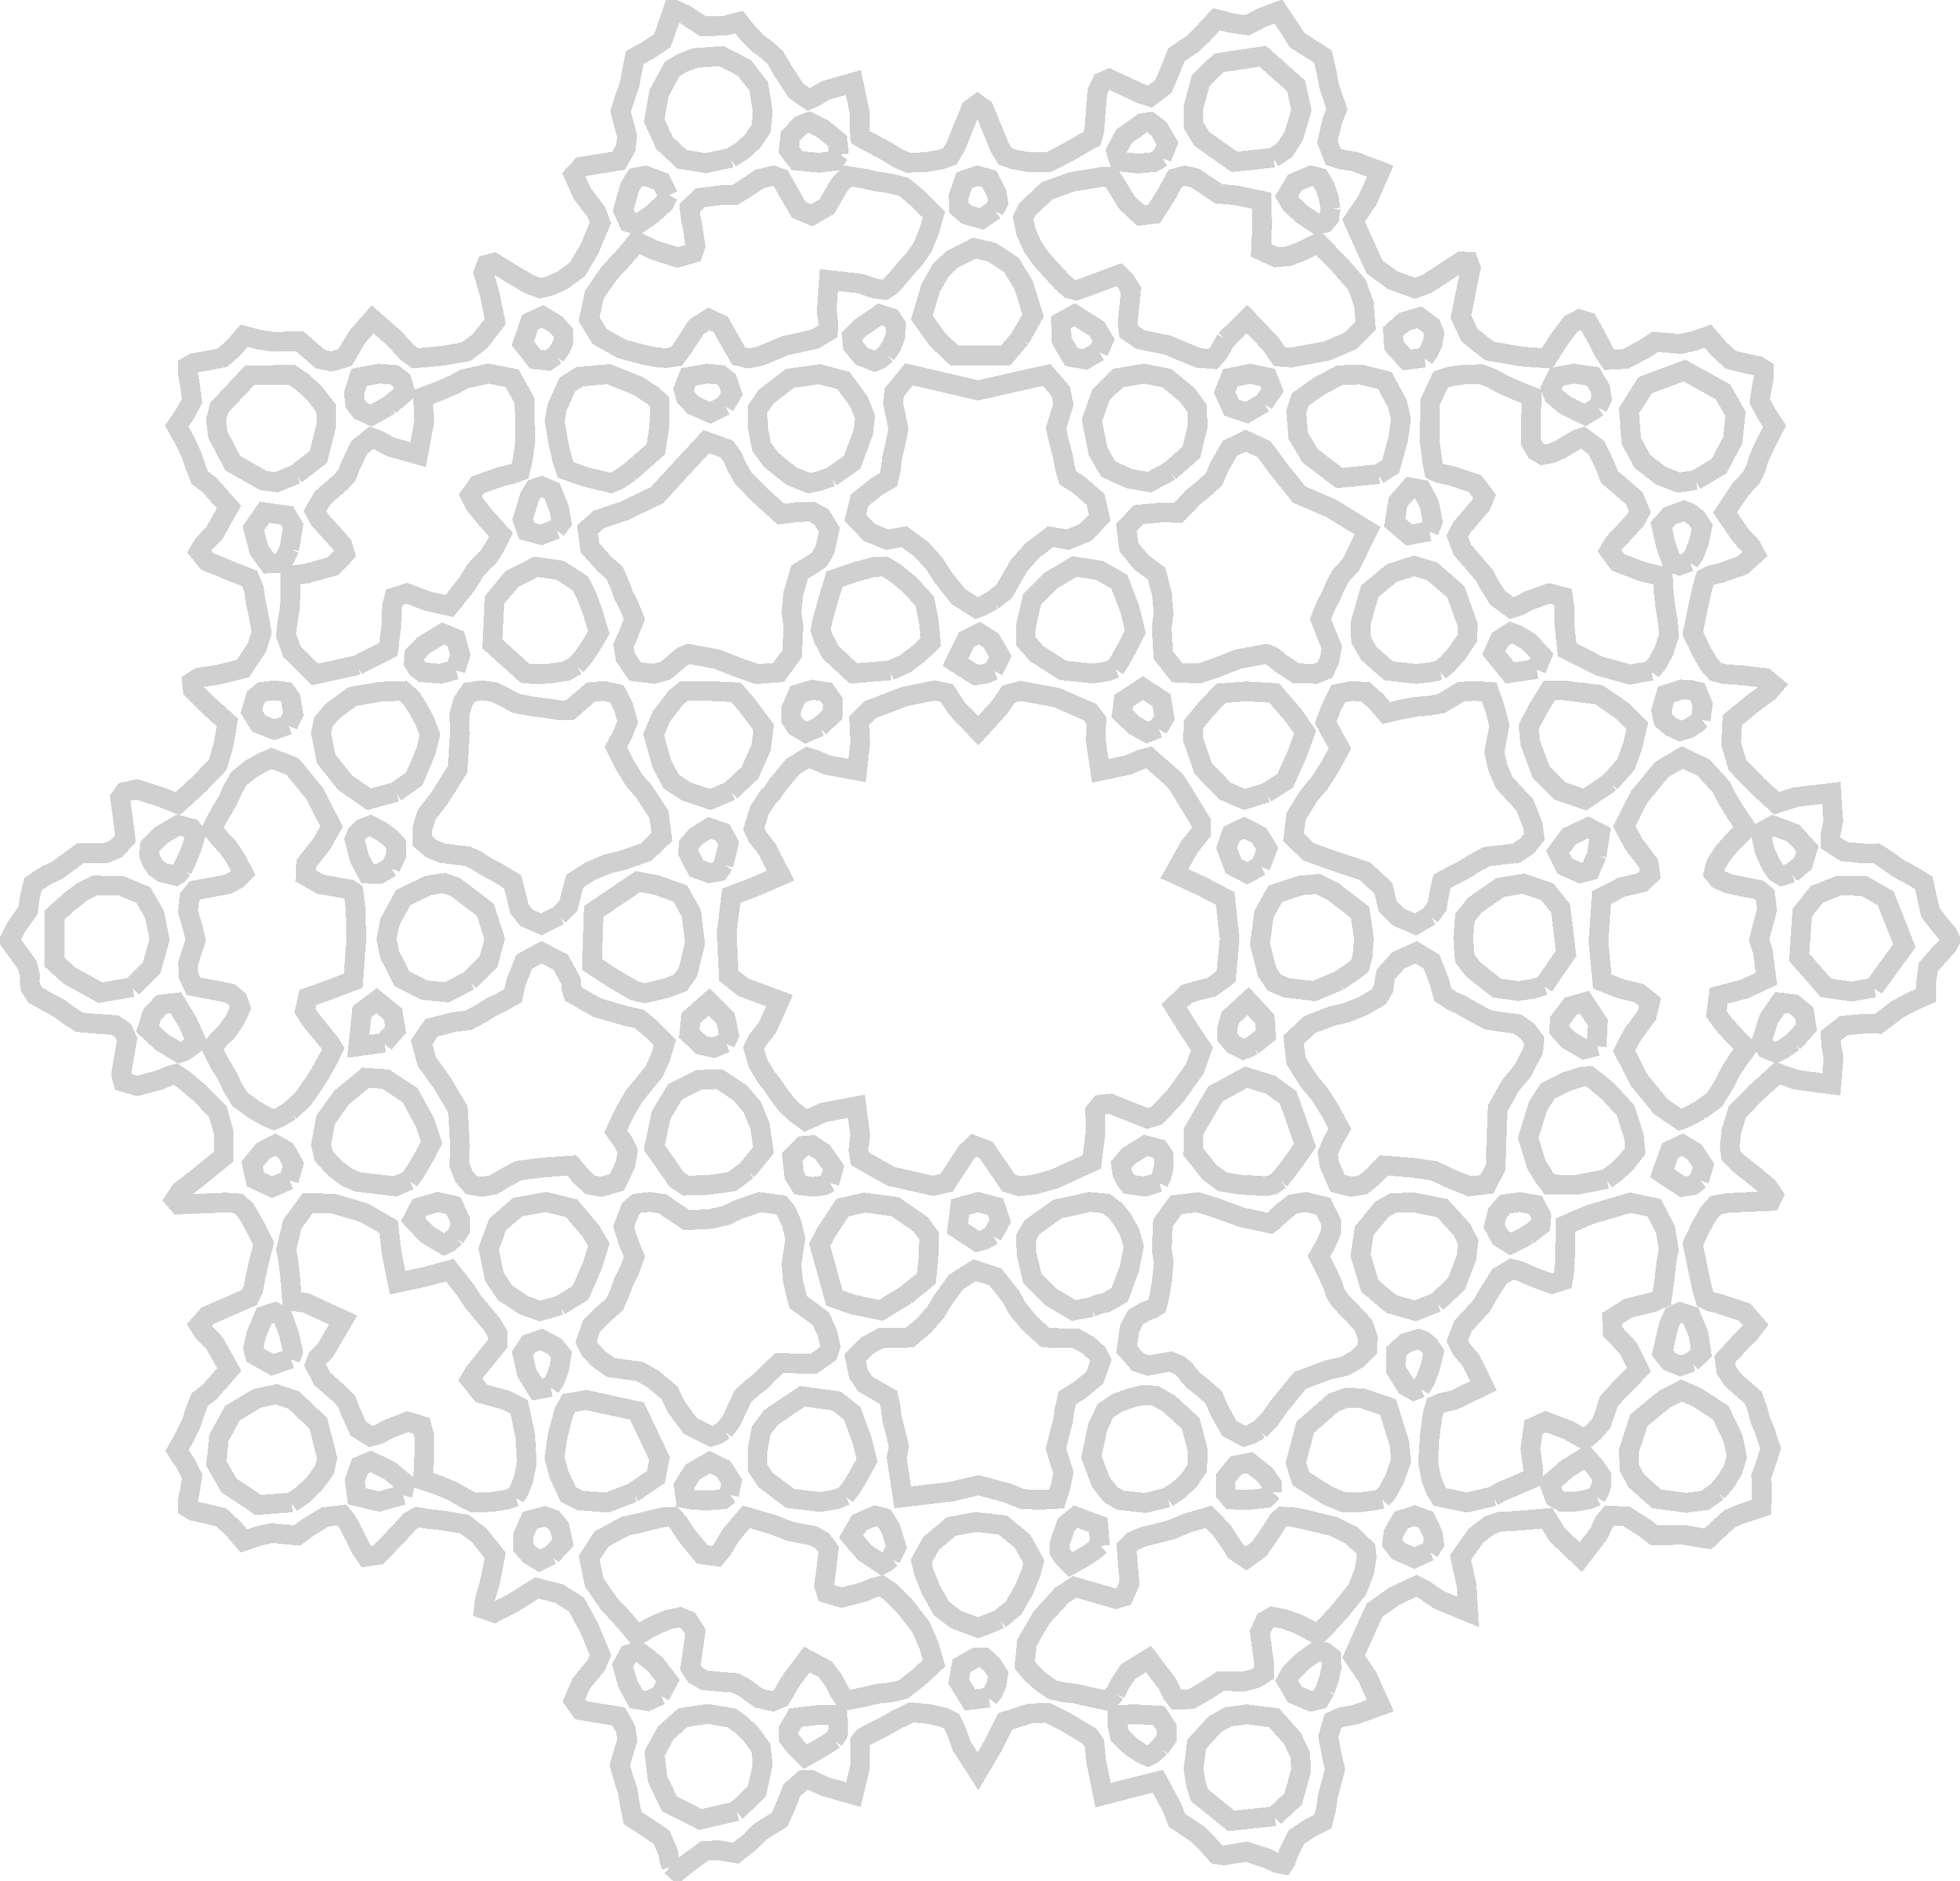
\includegraphics[width=1\textwidth]{./qq552.pdf}
\end{minipage}\hspace{1em}
\begin{minipage}{0.2\textwidth}
\end{minipage}
\begin{minipage}{0.8\textwidth}
{\Huge \bfseries Quasicrystals}\\
\HRule\\
\end{minipage}
\vspace{10 mm}


A five-fold quasicrystaline geometry underlies these ornaments. Quasicrystals are full of emergent, fractal patterns, but are simple to describe. A crystal is a structure that repeats. A quasicrystal is a structure that \emph{almost} repeats. Two dimensional quasicrystals can be built by superimposing simple patterns of stripes. Lets start with a one dimensional crystal. This is a repeating pattern of stripes:
\begin{figure}[H]\centering
$\begin{array}{l}
\includegraphics[width=.1\textwidth,keepaspectratio]{1_grey.png}\end{array}$
\end{figure}
Two waves, at right angles, makes a checkerboard:
\begin{figure}[H]\centering
$\begin{array}{l}
\includegraphics[width=.1\textwidth,keepaspectratio]{2_0_grey.png}\end{array}$+
$\begin{array}{l}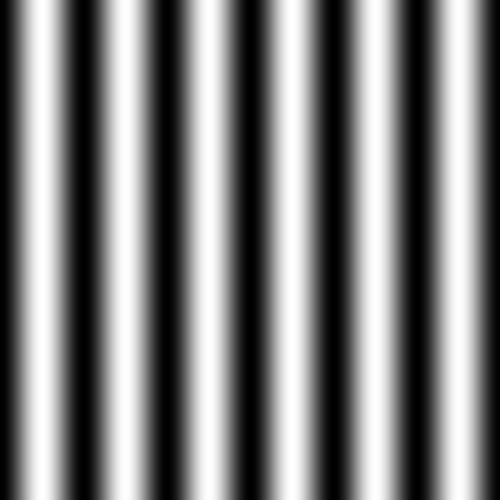
\includegraphics[width=.1\textwidth,keepaspectratio]{2_1_grey.png}\end{array}$=
$\begin{array}{l}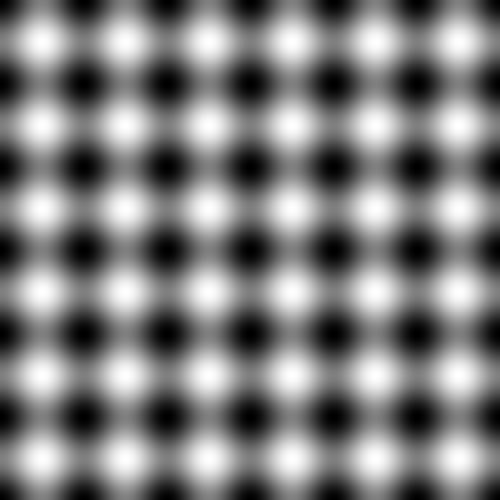
\includegraphics[width=.1\textwidth,keepaspectratio]{2_grey.png}\end{array}$
\end{figure}
Three waves, equally spaced in three different directions, makes a repeating honeycomb:
\begin{figure}[H]\centering
$\begin{array}{l}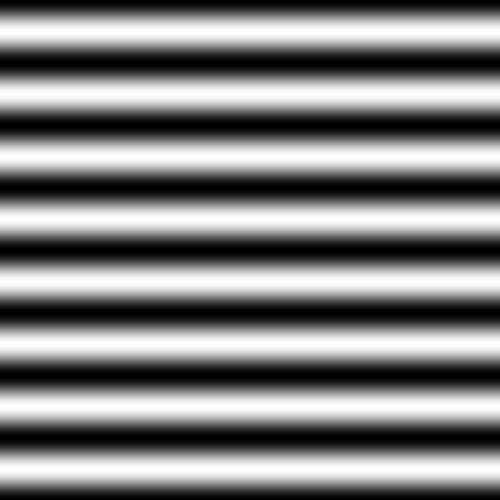
\includegraphics[width=.1\textwidth,keepaspectratio]{3_0_grey.png}\end{array}$+
$\begin{array}{l}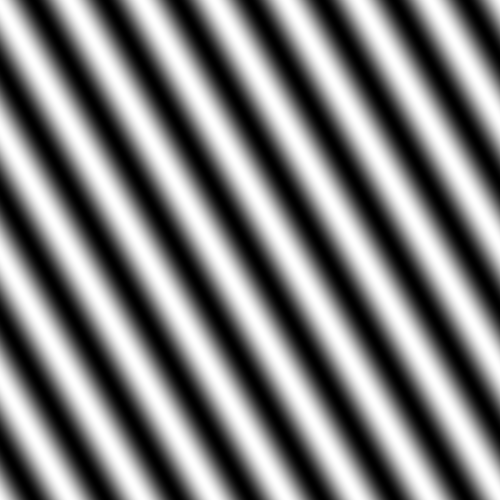
\includegraphics[width=.1\textwidth,keepaspectratio]{3_1_grey.png}\end{array}$+
$\begin{array}{l}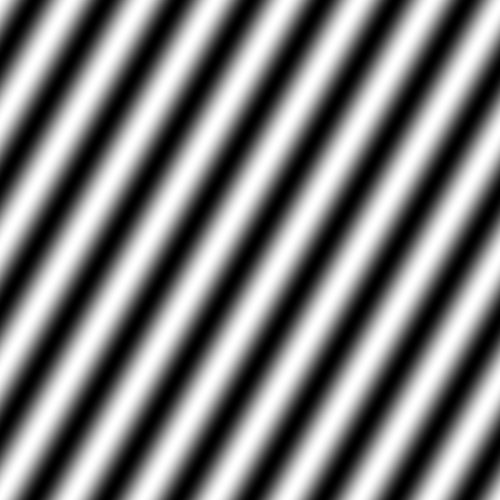
\includegraphics[width=.1\textwidth,keepaspectratio]{3_2_grey.png}\end{array}$=
$\begin{array}{l}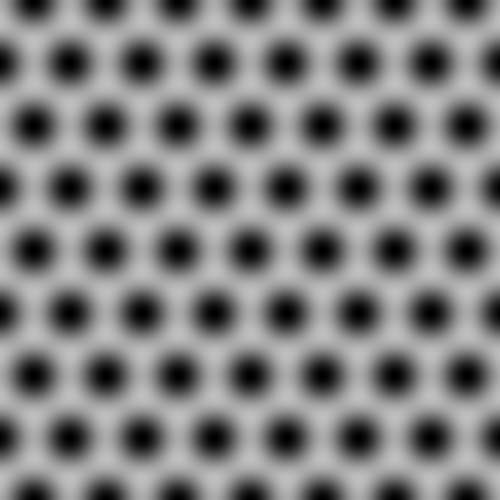
\includegraphics[width=.1\textwidth,keepaspectratio]{3_grey.png}\end{array}$
\end{figure}
Something interesting happens when we go to four waves though: the waves no longer overlap in a simple, repeating pattern:
\begin{figure}[H]\centering
$\begin{array}{l}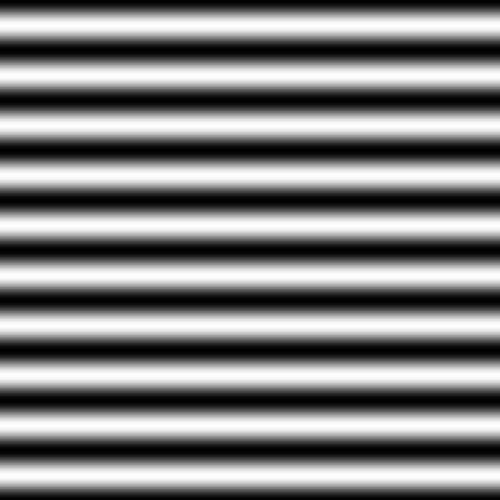
\includegraphics[width=.1\textwidth,keepaspectratio]{4_0_grey.png}\end{array}$+
$\begin{array}{l}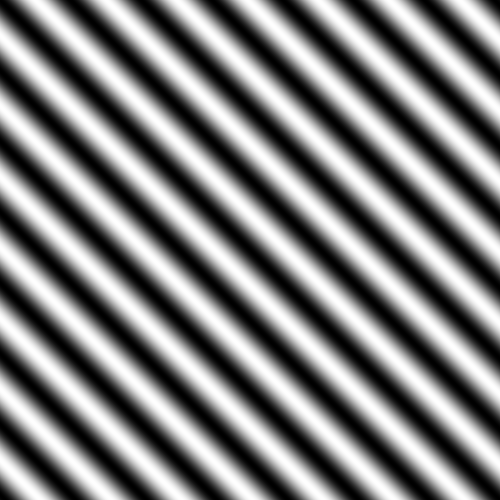
\includegraphics[width=.1\textwidth,keepaspectratio]{4_1_grey.png}\end{array}$+
$\begin{array}{l}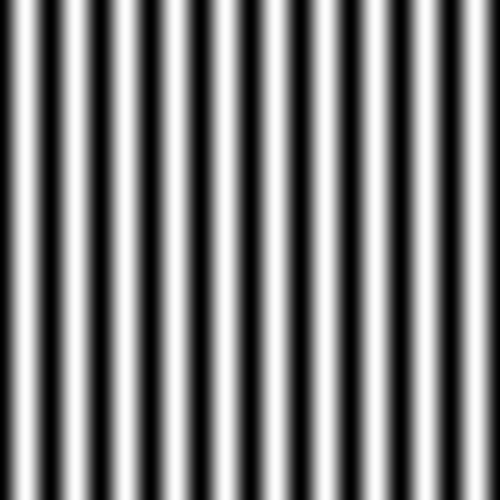
\includegraphics[width=.1\textwidth,keepaspectratio]{4_2_grey.png}\end{array}$+
$\begin{array}{l}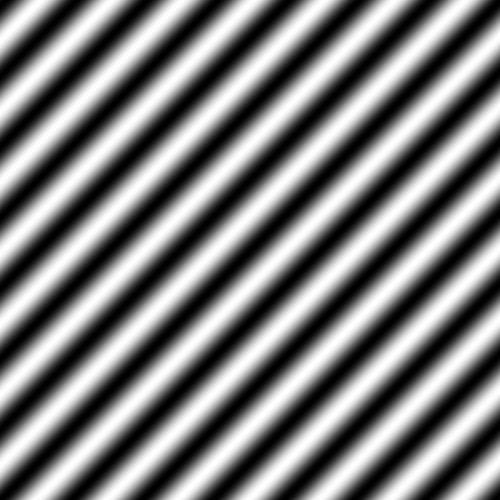
\includegraphics[width=.1\textwidth,keepaspectratio]{4_3_grey.png}\end{array}$=
$\begin{array}{l}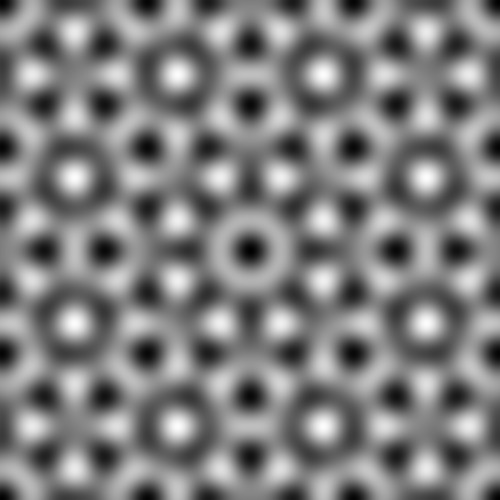
\includegraphics[width=.1\textwidth,keepaspectratio]{4_grey.png}\end{array}$
\end{figure}
These designs are based on the five-fold two dimensional quasicrystal:
\begin{figure}[H]\centering
$\begin{array}{l}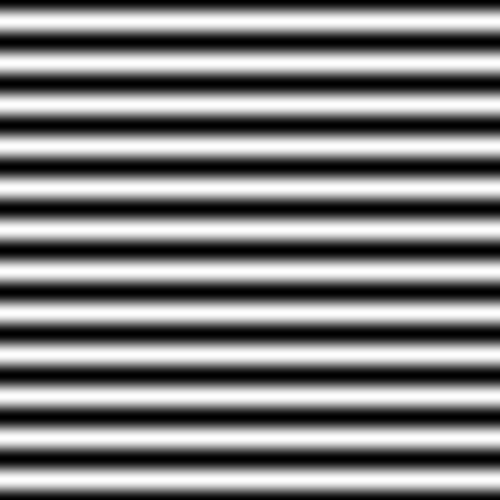
\includegraphics[width=.1\textwidth,keepaspectratio]{5_0_grey.png}\end{array}$+
$\begin{array}{l}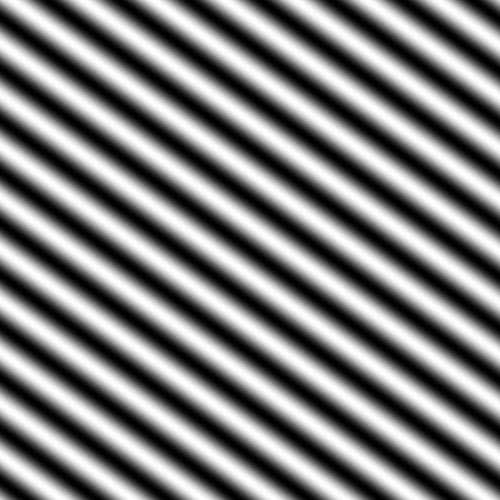
\includegraphics[width=.1\textwidth,keepaspectratio]{5_1_grey.png}\end{array}$+
$\begin{array}{l}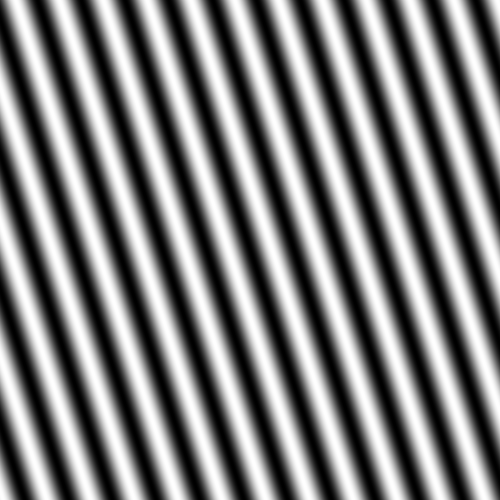
\includegraphics[width=.1\textwidth,keepaspectratio]{5_2_grey.png}\end{array}$+
$\begin{array}{l}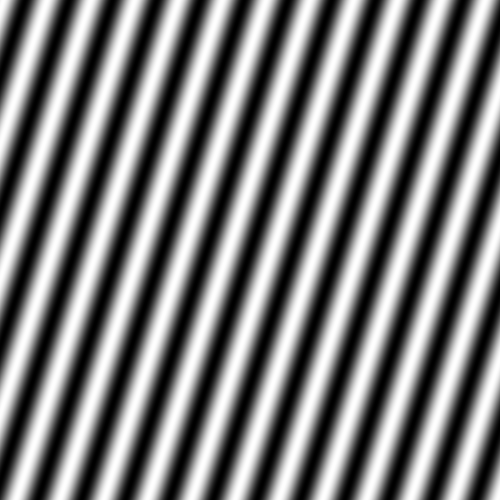
\includegraphics[width=.1\textwidth,keepaspectratio]{5_3_grey.png}\end{array}$+
$\begin{array}{l}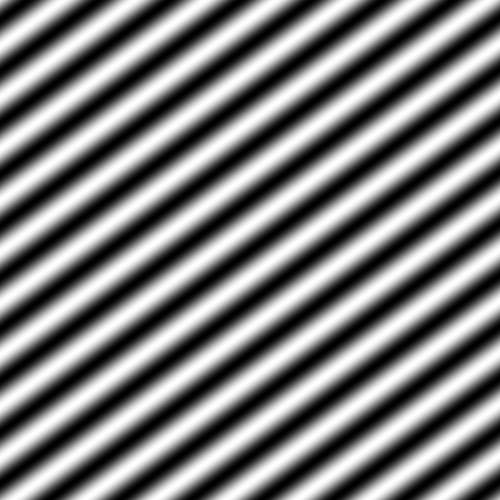
\includegraphics[width=.1\textwidth,keepaspectratio]{5_4_grey.png}\end{array}$=
$\begin{array}{l}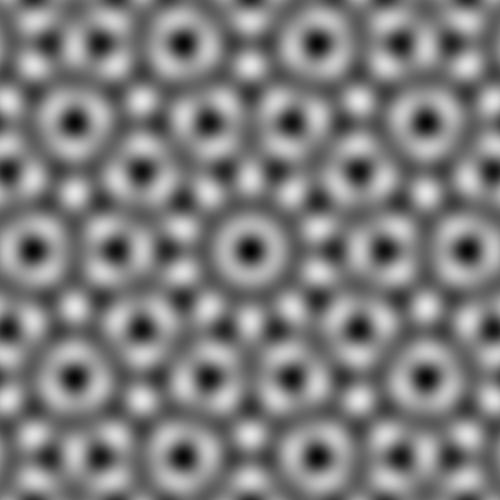
\includegraphics[width=.1\textwidth,keepaspectratio]{5_grey.png}\end{array}$
\end{figure}
Three dimensional quasicrystals are also possible, but are more complicated. They can be thought of as slices through higher-dimensional crystals. Many metal alloys naturally form quasicrystals, and the discovery of natural quasicrystals was the subject of the 2011 Nobel prize in chemistry. 


\end{document}